\chapter{Theory}

\section{Acoustic waves and waveguides}

In order to efficiently model the deformation and stresses in a solid material,
a linear elasticity model is often assumed.
For small deformations, solid materials obey Hooke's law which in it's full form
looks like
\[
	\sigma = C : \epsilon
\]
where $\sigma$ is the stress tensor, $C$ the elasticity tensor which is a
four-tensor that is a property of the material,
$\epsilon \coloneqq \nabla \vec u + (\nabla \vec u)^\transpose$
is the strain tensor, and $:$ denotes double scalar product.
This equation is linear in $\vec u$, hence the name \emph{linear} elasticity.
Using this and newtons equations of motion, the equation governing the dynamics
is obtained:
\[
	\rho \ddot{\vec{u}} = \nabla \cdot \sigma + \vec F.
\]
where $\rho$ is the density, $\vec{u}$ is the displacement and $\vec F$ is the
externally applied force.
Assuming a time harmonic solution
$\vec u(\vec x, t) = \vec u(x) e^{i \omega t}$
with angular frequency $\omega$ this becomes
\[
	-\rho \omega^2 \vec{u} = \nabla \cdot \sigma + \vec F.
\]

To combine these into one equation that can be solved for $\vec{u}$ we first
rewrite them in index notation to make calculations clearer:
\begin{align}
	\epsilon_{ij} &= \frac12(\partial_i u_j + \partial_j u_i)\\
	\sigma_{ij} &= C_{ijkl} \epsilon_{kl}\\
				&= \frac12\left(C_{ijkl} \partial_k u_l + C_{ijkl} \partial_l
				u_k\right)\\
				&= C_{ijkl} \partial_k u_l\text{ because of the symmetry of $C$}
\end{align}
which gives
\begin{align}
	F_{i} &= -\rho \omega^2 u_{i} - \partial_j \sigma_{ij}\\
		   &= -\rho \omega^2 \delta_{ik} u_{k} -
		   \partial_j \left(C_{ijkl} \partial_l u_k\right)\\
		   &= -\left(\rho \omega^2 \delta_{ik} \placeholder + 
		   \partial_j \left(C_{ijkl} \partial_l \placeholder\right)\right) u_k
\end{align}
where the indices $i,j,k,l$ go over the spacial dimensions $x,y,z$.
All of the tensors in the equation above are really tensor fields, i.e.\ they are
functions of $\vec{x}$.
Defining the operator $\hat A_{ik}$ as
$-\left(\rho \omega^2 \delta_{ik} \placeholder + 
\partial_j \left(C_{ijkl} \partial_l \placeholder\right)\right)$
we can write
\begin{equation}\label{eq:gov_eq}
	\hat A_{ik} u_k = F_i
\end{equation}

\todowrt{
With no external forces we get traveling modes=eigenvalues.
Explain how and why periodicity means only certain modes can propagate.
Good resource in Chan's thesis, or maybe solid state physics book?
% Bloch state / Bloch's theorem
}
\subsection{Bloch States and Band Diagrams}

With no external forces, i.e.\ $F_i = 0$, \cref{eq:gov_eq} can be written as
\begin{equation}
	\frac 1 \rho \partial_j \left(C_{ijkl} \partial_l u_k\right) = \omega^2 u_i
\end{equation}
which is an eigenvalue equation for the operator
$\hat O_{ik} = \frac 1 \rho\partial_j \left(C_{ijkl} \partial_l \placeholder\right)$
where eigenvalues are the angular frequency squared.
If furthermore the structure is periodic, then the eigenstates are so called
\emph{Bloch states}.

If the structure is periodic with some periodicity $\vec a$,
meaning that $C_{ijkl}(\vec x) = C_{ijkl}(\vec x + n \vec a)$ where $n$ is an
integer, then this operator commutes with the translation operator
$\hat T_{\vec a} \vec u(\vec x) = \vec u(\vec x + \vec a)$.
This means that there is a space of simultaneous eigenstates to both of them.
The eigenfunctions of the translation operator are $\exp(i \vec k \cdot \vec
x)$ with eigenvalues $\exp(i k a)$, where $a = \abs{a}$.
Defining the reciprocal lattice constant $\vec b = 2 \pi \vec a / a^2$, we see
that the functions $\exp(i (\vec k + m \vec b) \cdot \vec x)$ for integer values
of $m$ all have the same eigenvalue, which means that they form a degenerate
subspace of eigenfunctions.
Thus we can write the eigenfunctions of both operators as
\begin{equation}
	\vec u_{\vec k}(\vec x) = \sum_m e^{i (\vec k + m \vec b) \cdot \vec x}
	\vec u_{m, \vec k}(\vec x)
	= e^{i \vec k \cdot \vec x} \bar{\vec u}_{\vec k}(\vec x)
\end{equation}
where $\bar{\vec{u}}_{\vec{k}}$ is a periodic function with periodicity $\vec a$.
\todocit[inline]{%
	Sakurai does basically the same derivation but for electronic
	states in a crystal lattice, but he also uses operator formalism. Can I cite
	that? Other option is citing Chan's PhD who do it the same way for photonic
	crystals and says that it can be done analogously for phononic crystals.
}

The solutions to these eigenvalue equations are often called modes, and each
mode has both a frequency and a wave vector. This gives rise to a band diagram,
where the frequency is plotted as a function of the wave vector.

\subsubsection{Concrete example of phononic crystal}

In this work, a rectangular waveguide patterned with ellipses is used.
The structure is clamped at the bottom (meaning that we use a fixed boundary
condition there) while the other sides are free.
A top down schematic of the unit cell can be seen in \cref{fig:unitcell}.

\begin{figure}[htpb]
\begin{center}
	\begin{tikzpicture}[scale=6]
	\def \a{0.5}
	\def \w{1.0}
	\def \hx{0.13}
	\def \hy{0.3}
	\def \fadedist{0.15}

	\draw[ultra thick] (-0.5*\w, -0.5*\a) rectangle (0.5*\w, 0.5*\a);
	\draw[ultra thick] (0, 0) circle [x radius=\hy, y radius=\hx];
	\draw[ultra thick, path fading=south]
		(-0.5*\w, -0.5*\a-\fadedist) --
		(-0.5*\w, -0.5*\a)
		(+0.5*\w, -0.5*\a) --
		(+0.5*\w, -0.5*\a-\fadedist);
	\draw[ultra thick, path fading=north]
		(-0.5*\w, 0.5*\a+\fadedist) --
		(-0.5*\w, 0.5*\a)
		(+0.5*\w, 0.5*\a) --
		(+0.5*\w, 0.5*\a+\fadedist);
	\draw[<->]
		(0.4*\w, -0.5*\a*0.95) -- node[right] {$a$}
		(0.4*\w, 0.5*\a*0.95);
	\draw[<->]
		(-0.5*\w*0.95, 0.6*\a) -- node[above] {$w$}
		(0.5*\w*0.95, 0.6*\a);
	\draw[<->] (0,0) -- node[right] {$h_y$} (0.0, 0.95*\hx);
	\draw[<->] (0,0) -- node[below] {$h_x$} (0.95*\hy, 0);
\end{tikzpicture}
\end{center}
\caption{Top down view of unit cell of a phononic crystal.}%
\label{fig:unitcell}
\end{figure}

Enforcing a wave vector $\vec k = k\hat{\vec y}$ and running COMSOL to find the eigenmodes with their
corresponding frequencies for this structure yields the band diagram in
\cref{fig:banddiagram}.
\Cref{fig:modeshapes} shows the shapes of the eight lowest lying eigenmodes at
$k=0.9 \pi / a$.
\begin{figure}[htpb]
	\centering
	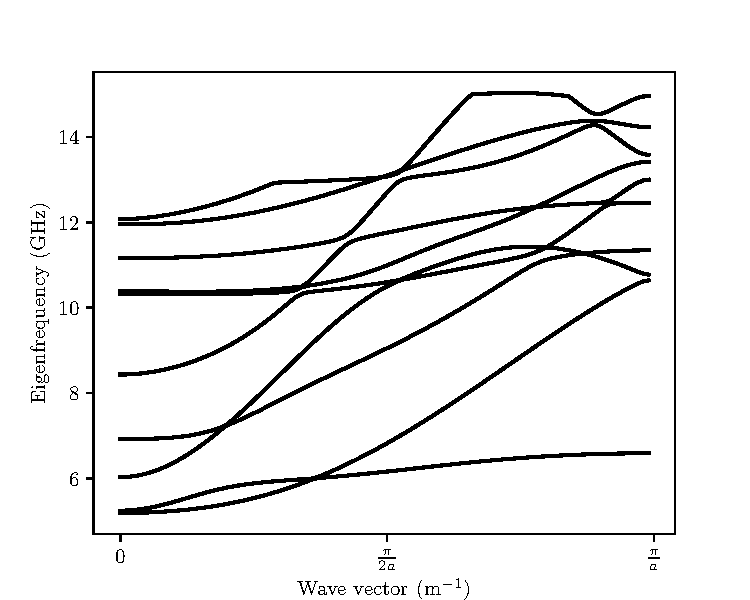
\includegraphics{chapters/theory/bandstructure.pdf}
	\caption{
		Band diagram of phononic crystal defined in \cref{fig:unitcell}.
	}%
	\label{fig:banddiagram}
\end{figure}

\begin{figure}[htpb]
	\centering
	\begin{subfigure}[]{0.24\textwidth}
		\begin{center}
			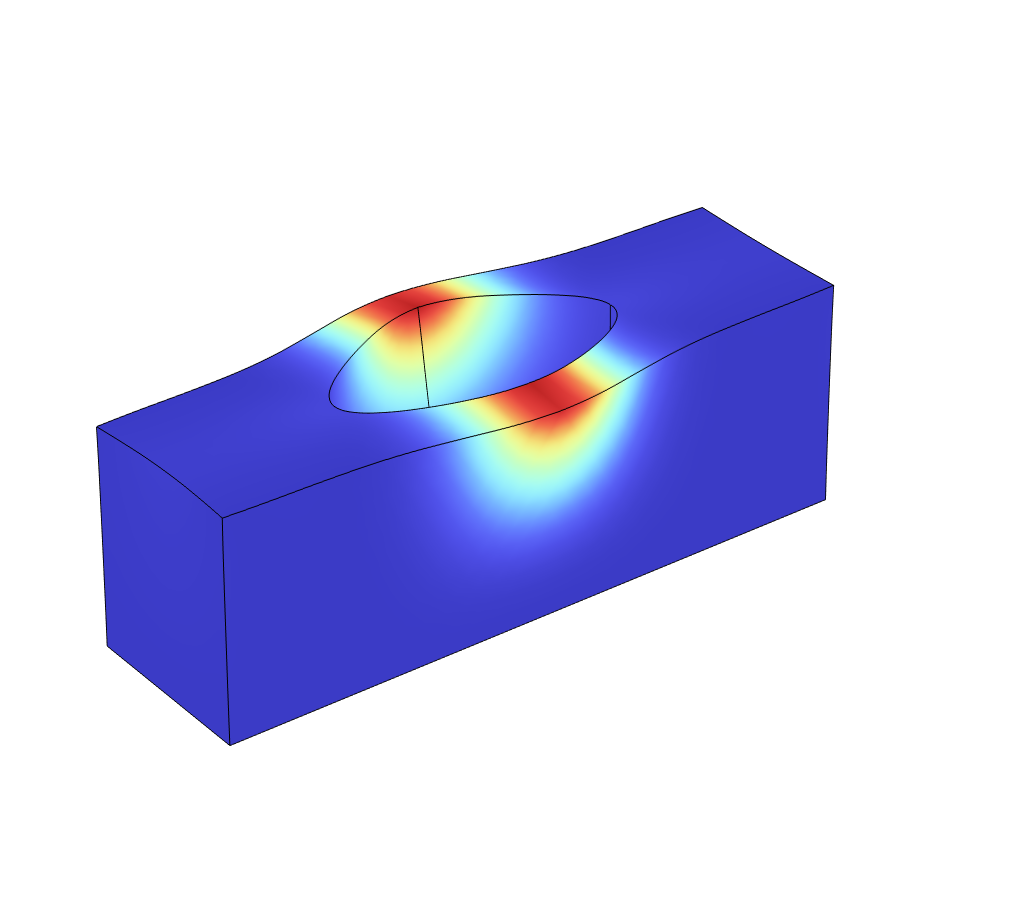
\includegraphics[width=\textwidth]{chapters/theory/modeshape_1.png}
		\end{center}
		\subcaption{}%
		\label{fig:ms1}
	\end{subfigure}
	\begin{subfigure}[]{0.24\textwidth}
		\begin{center}
			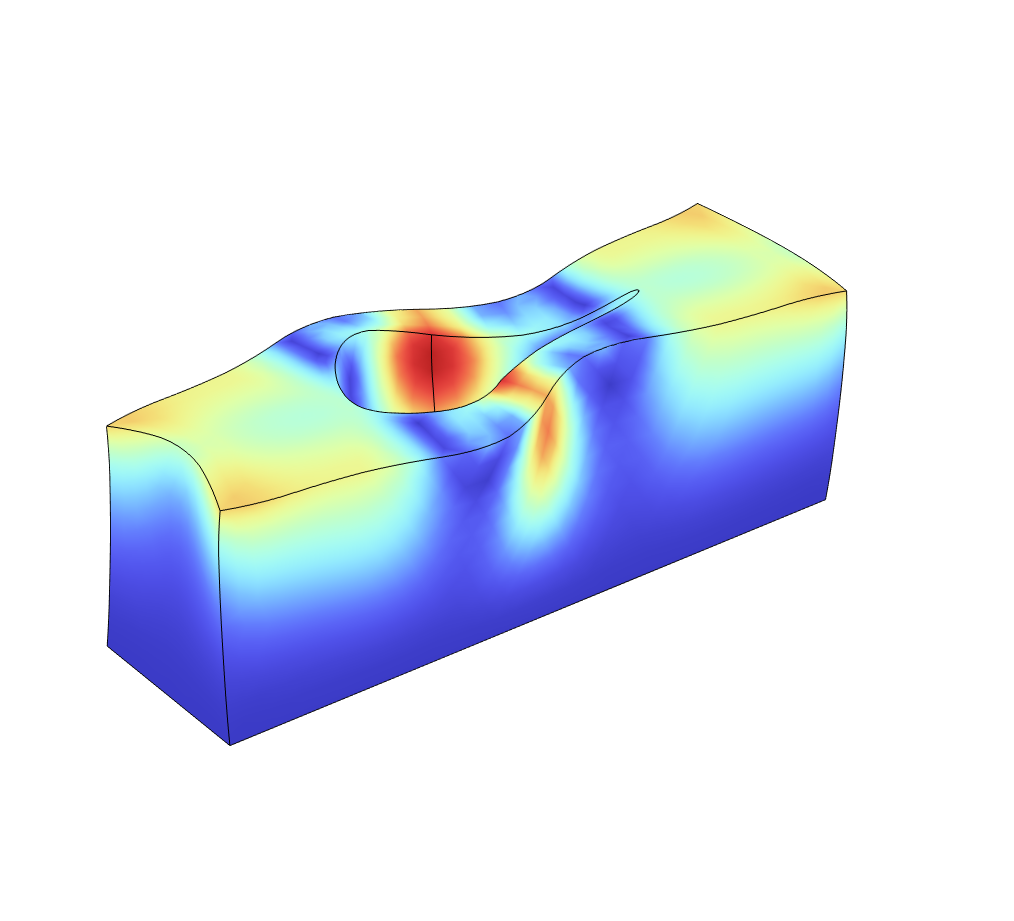
\includegraphics[width=\textwidth]{chapters/theory/modeshape_2.png}
		\end{center}
		\subcaption{}%
		\label{fig:ms2}
	\end{subfigure}
	\begin{subfigure}[]{0.24\textwidth}
		\begin{center}
			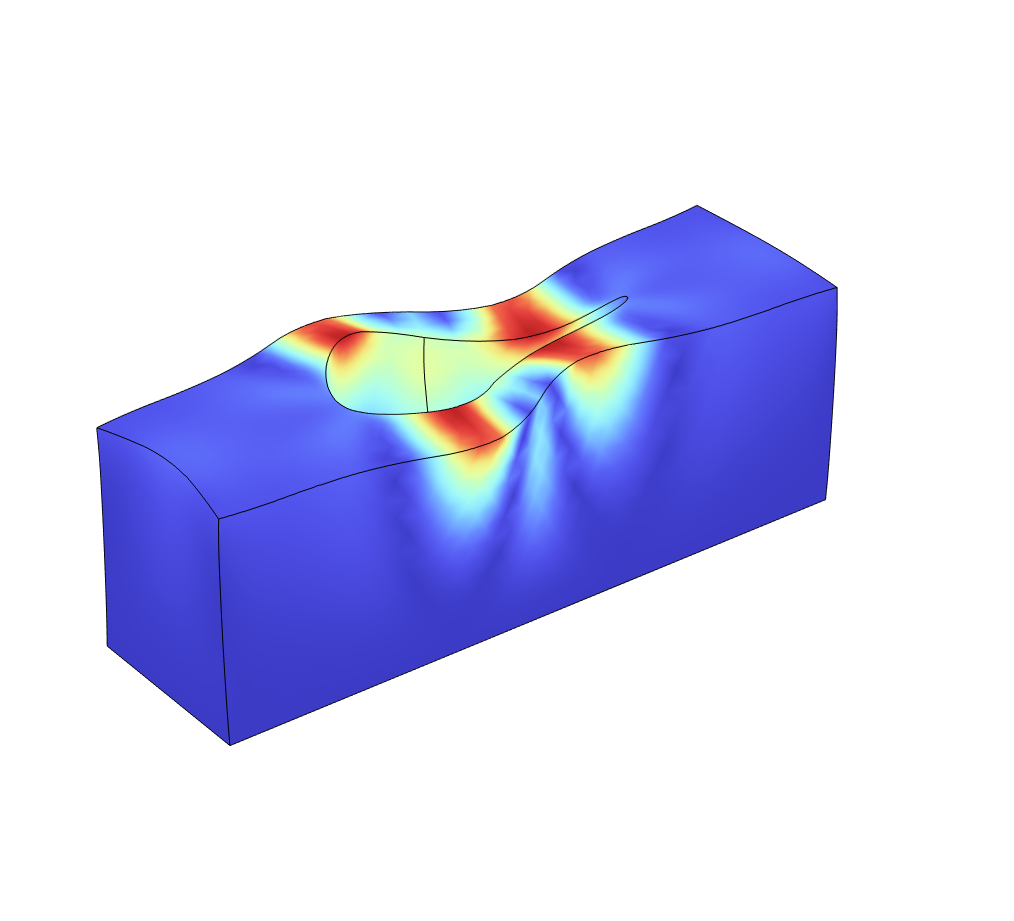
\includegraphics[width=\textwidth]{chapters/theory/modeshape_3.png}
		\end{center}
		\subcaption{}%
		\label{fig:ms3}
	\end{subfigure}
	\begin{subfigure}[]{0.24\textwidth}
		\begin{center}
			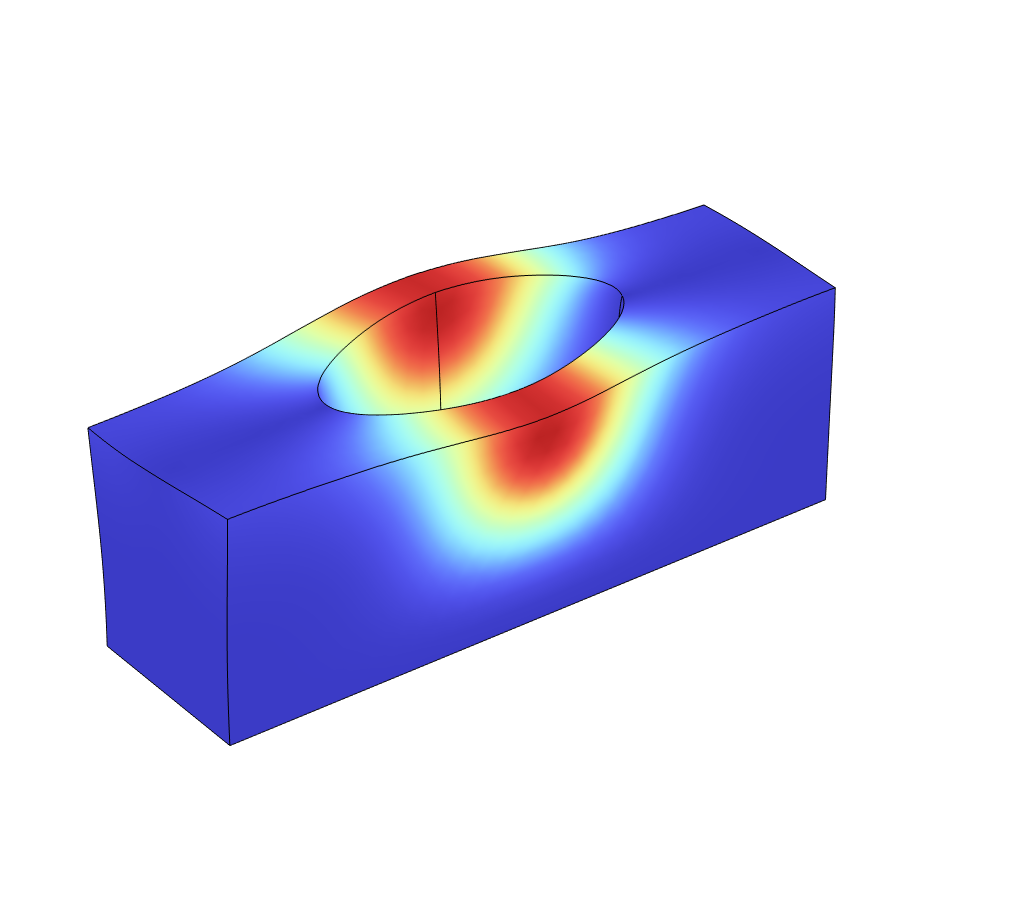
\includegraphics[width=\textwidth]{chapters/theory/modeshape_4.png}
		\end{center}
		\subcaption{}%
		\label{fig:ms4}
	\end{subfigure}\\

	\begin{subfigure}[]{0.24\textwidth}
		\begin{center}
			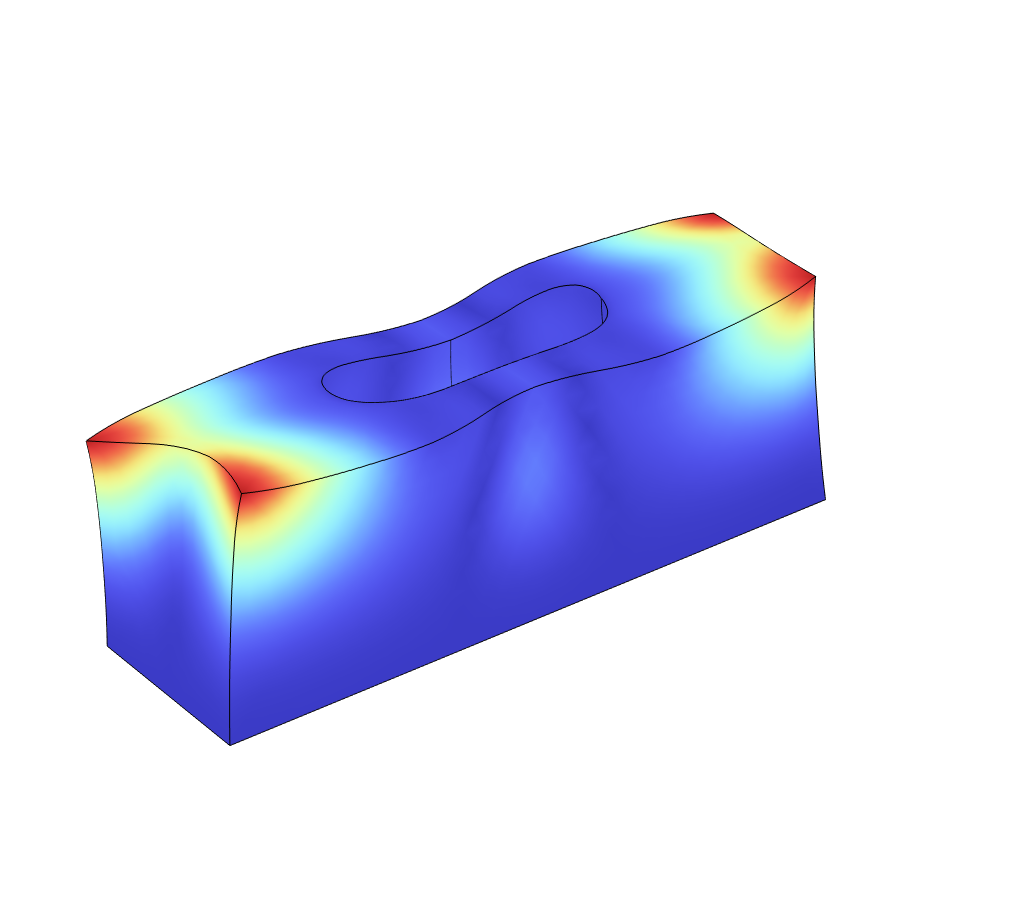
\includegraphics[width=\textwidth]{chapters/theory/modeshape_5.png}
		\end{center}
		\subcaption{}%
		\label{fig:ms5}
	\end{subfigure}
	\begin{subfigure}[]{0.24\textwidth}
		\begin{center}
			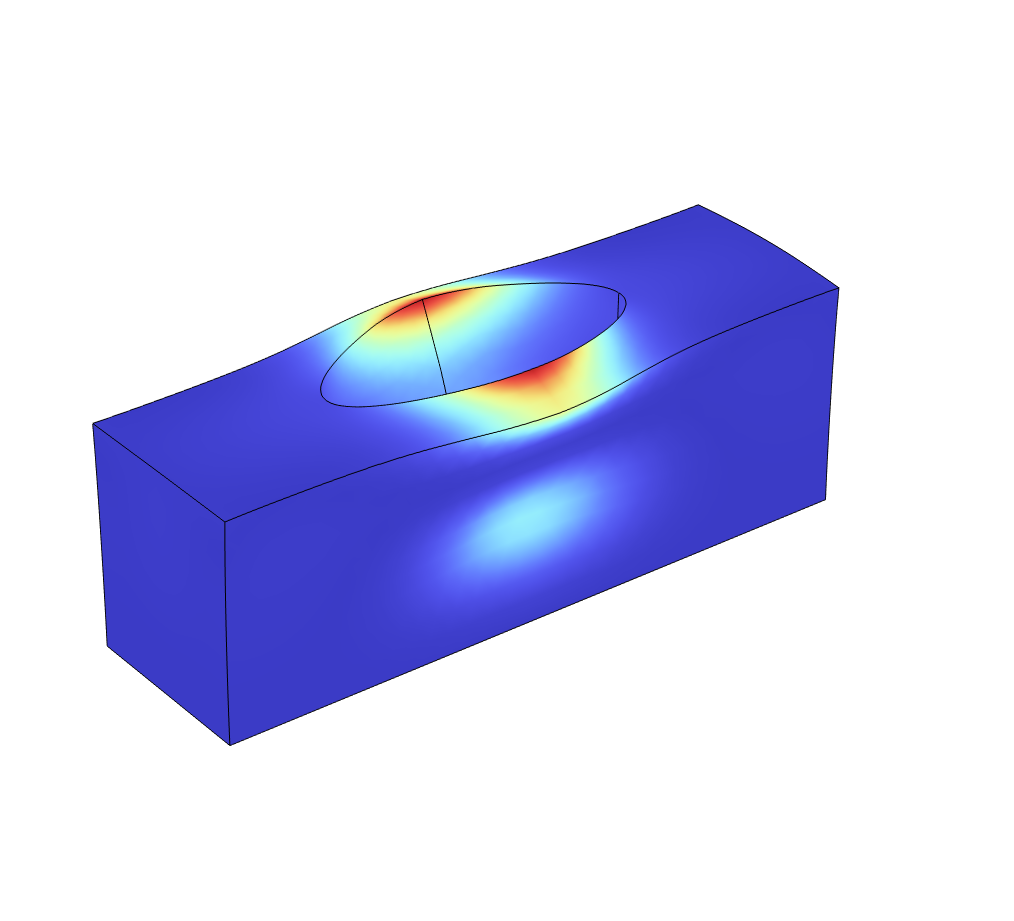
\includegraphics[width=\textwidth]{chapters/theory/modeshape_6.png}
		\end{center}
		\subcaption{}%
		\label{fig:ms6}
	\end{subfigure}
	\begin{subfigure}[]{0.24\textwidth}
		\begin{center}
			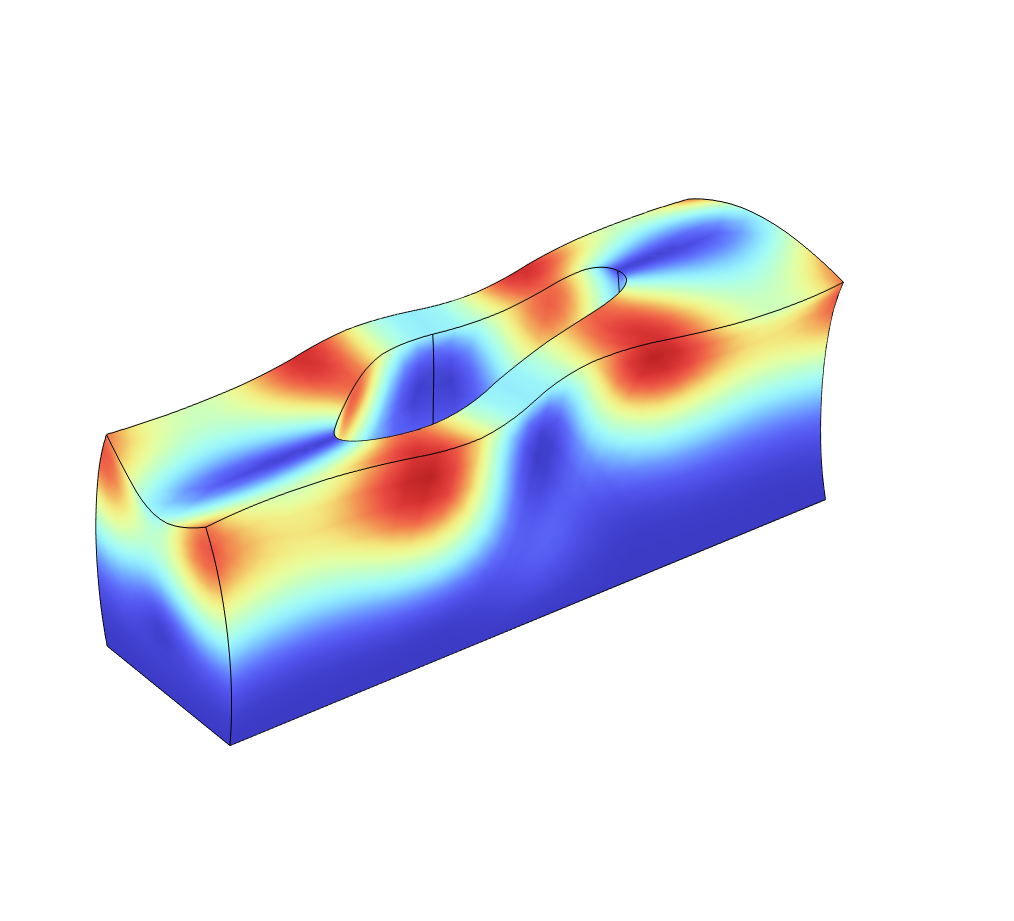
\includegraphics[width=\textwidth]{chapters/theory/modeshape_7.png}
		\end{center}
		\subcaption{}%
		\label{fig:ms7}
	\end{subfigure}
	\begin{subfigure}[]{0.24\textwidth}
		\begin{center}
			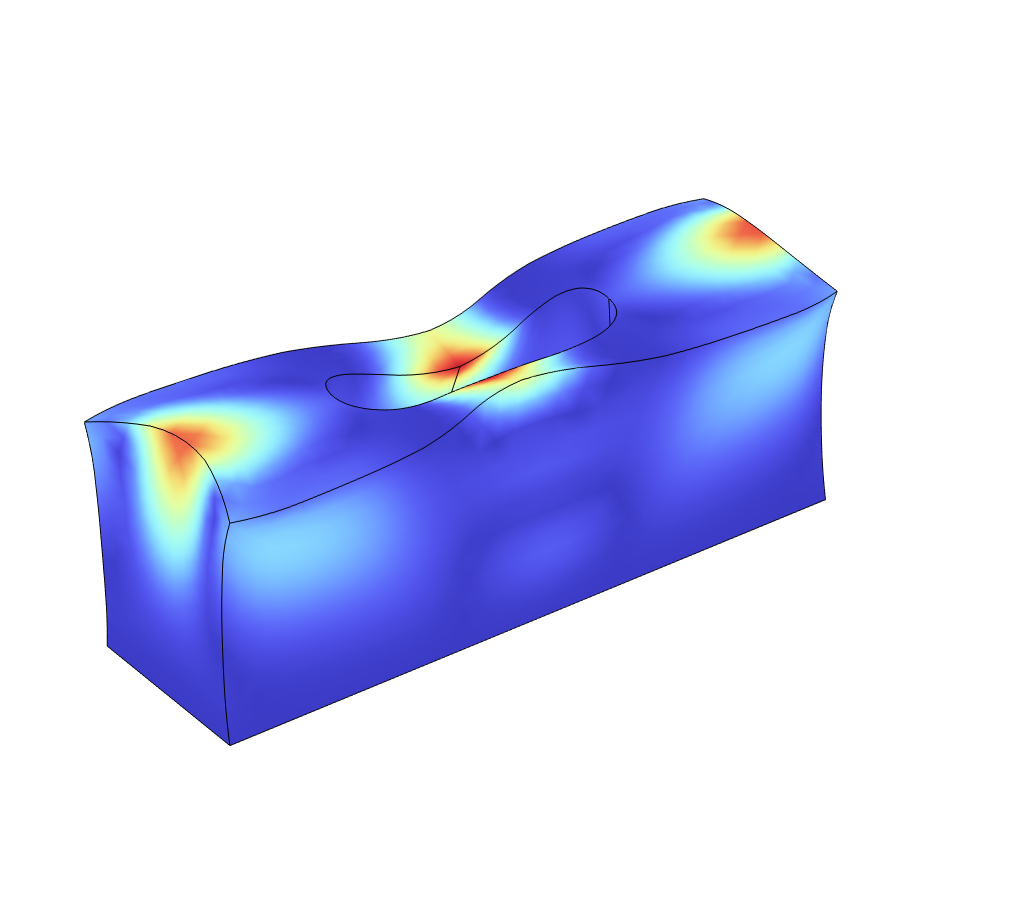
\includegraphics[width=\textwidth]{chapters/theory/modeshape_8.png}
		\end{center}
		\subcaption{}%
		\label{fig:ms8}
	\end{subfigure}

	\caption{%
		Mode shapes for the lowest eight modes at $k=0.9 \pi / a$.
		The color denotes the absolute value of the displacement.
	}
	\label{fig:modeshapes}
\end{figure}
\tododec{At some point write about phonons? I haven't really had to care about
the fact that excitations are discrete so if I talk about it it'd just for applications...}

\todowrt{Write about PML design and why we need it: Simulating infinite
	waveguides isn't possible because of the finite computing power. Also we
don't care about stuff far away, just that there are no reflections that can
interfere. Or maybe write about this in the method\ldots}

\section{Inverse Design}

Inverse design is a design paradigm where the design of a device is guided fully by
the desired characteristics.
These desired characteristics are quantified through what is called an objective
function%
\footnote{
	Also called \emph{figure of merit (FoM)} by some.%
}%
, which I will denote $\fobj$,
that should be maximized.
When coupled with \emph{adjoint simulation}, which is a clever way to compute
gradients, and gradient based optimization
algorithms, this is a very powerful methodology.

An overview of the design process is as follows:
\begin{enumerate}
	\item Initialize a random device design.
	\item\label{it:grad} Calculate the gradient of the design through the adjoint method.
	\item Update the device design using the gradient according to the optimization algorithm.
	\item If the device performance is good enough, terminate optimization, else
		return to step~\ref{it:grad}.
\end{enumerate}

\subsection{Adjoint Simulation}

Adjoint simulation is a way to compute the gradient of $\fobj$ with respect to
the design, which in our case means with respect to the material parameters.
I will in this section first give a general derivation, followed by the case of
inverse design in acoustics.

\subsubsection{General Derivation}\label{sec:general_derivation}

Let $\fobj$ be a function which depends on some (large) vector $v$.
The vector $v$ can be calculated by solving the linear equation
$A v = b$, where $b$ is a fixed vector and $A$ is a matrix that depends on a
vector of design parameters $p$.
The overall goal is to find the parameters $p$ that maximize the objective
function $\fobj$.
The goal of adjoint simulation is to find $\diff{\fobj}{p}$.
This can be expanded through the chain rule as
\[
	\diff{\fobj}{p} = \diff{\fobj}{v} \diff{v}{p}.
\]
To find the latter factor we do
\begin{align*}
	\diff{}{p} [Av = b] &\implies \diff{A}{p} v + A \diff{v}{p} = 0\\
						&\implies \diff{v}{p} = -A^{-1} \diff{A}{p} v
\end{align*}
which gives
\begin{align}
	\diff{\fobj}{p} &= - \diff{\fobj}{v} A^{-1} \diff{A}{p}
	v\label{eq:no_adj_sim}\\
	&= - \left(A^{-T} \diff{\fobj}{v}^\transpose \right)^\transpose \diff{A}{p} v
\end{align}
The first factor of this product is the solution to the \emph{adjoint problem}
\begin{equation}
	A^\transpose \tilde v = \diff{\fobj}{v}^\transpose,
\end{equation}
hence the name adjoint simulation.
As it turns out, $A$ is often symmetric (or self-adjoint) which means that this is simply a normal
simulation but with $\difs{\fobj}{v}^\transpose$ (or $\difs{\fobj}{v}^\dagger$) as the source.
Thus, to obtain the derivative we just need to run an additional
simulation with a different input.

Now you might be wondering: what have we gained by this?
Let $n$ be the dimension of $v$, $m$ the dimension of $p$ and $l$ the dimension
of $b$.
This means that $A$ is a matrix with dimension $l\times n$ and $\difs{A}{p}$ is
a three-tensor with dimension $m\times l\times n$.
Thus calculating $A^{-1} \difs{A}{p}$ directly involves solving $Ax = w$ for a
three-tensor, and calculating $A^{-1} \left(\difs{A}{p}\,v\right)$
involves solving for a matrix, both of which are orders of magnitude more
computationally expensive than solving for a vector.

\subsubsection{Specific derivation with acoustics}\label{sec:spec_der}

Now we turn to the specific case of acoustic devices.
Here $A v = b$ is replaced by the dynamic equation \todowrt[noinline]{dynamic equation?
Better name} of linear elasticity:
\begin{equation}\label{eq:sim_eq}
	\hat A_{ik} u_k = F_i
\end{equation}
Instead of vectors, like we saw in \cref{sec:general_derivation}, these quantities are now functions%
\footnote{%
	Vector-valued funcitons, but that is not the important part here.
}
of $\vec x$.
Analogously to the vector of design parameters we now have a \emph{design field}
$p(\vec x)$.

\begin{tcolorbox}[title=On functionals and their derivatives, breakable,
	parbox=false]
	\tododec{
		Big fat box on functionals and their derivatives. I think this should be
		included somewhere, since very few of my peers know what a functional
		derivative is... Not really sure how though. I kinda like the thought of
		putting it in a box like this.
		Alternatively, I could put it in an appendix.
	}
Our $\fobj$ is no longer a function, but rather a \emph{functional}, and thus
we need to use the functional derivative instead of the ordinary derivative.
One can think of a functional as a function of a function,
i.e.\ something that maps an element of a function space to a scalar number.
There are also functionals which depend on both a function and a real number,
or on multiple functions.
Below I will give an overview of the notational conventions I use,
and then give the definition of the functional derivative as well as some useful
properties of it.

Let $\mathcal{Y}$ be a function space of functions $\R \to \R$.
A functional $F:\mathcal{Y} \to \R$ evaluated at the function
$f\in\mathcal{Y}$
is notated with the function in square brackets: $F[f]$.
Note that in principle, $F$ is the functional while $F[f]$ is just a
number,
analogously to how $f$ is a function while $f(x)$ is a real number.
If the functional additionally depends on a real number,
$G:\mathcal{Y} \times \R \to \R$,
that is put in round brackets: $G[f](x)$.

The functional derivative of $F$ with respect to it's function argument
is a functional $\mathcal{Y} \times \R \to \R$ denoted $\difs.f.{F[f]}{f}$.
In this expression, $f$ is technically a dummy function, writing
$\difs.f.{F[g]}{g}$ is exactly the same functional.
However, often the argument of $F$ is omitted and the function in the
denominator is named in accordance with the names in the definition of the
functional.
Furthermore, the same notation is also often used to denote the functional
derivative evaluated at a certain function.
For example, if we define a functional taking two function arguments
$F[f_1, f_2] = \int f_1(x) + f_2(x) \dl x$, one can write
\begin{align}
	\diff.f.{F}{f_2}(x)
	&& \text{meaning}&\quad \diff.f.{F[g_1, g_2]}{g_2}(x)\\
	\diff.f.{F}{f_2}(x)
	&& \text{meaning}&\quad \diff.f.{F[g_1, g_2]}{g_2} [f_1, f_2](x)
\end{align}
where in the latter case, $f_1$ and $f_2$ are specific functions defined
previously.
% Almost always the functional derivative will be evaluated
% at some function $h$.
% In proper notation this should be written
% \begin{equation}
% 	\diff.f.{F[g]}{g} [h]
% \end{equation}
% and is simply an ordinary function $\R \to \R$.
% However, I will use the notation $\difs.f.{F}{h}$ for this, to make the
% equations clearer. In addition, when evaluating the functional derivative at a point, the
% argument can be put either after it, or in the denominator:
% \begin{equation}
% 	\diff.f.{F[g]}{g} [h](x) = \diff.f.{F}{h}(x) = \diff.f.{F}{h(x)}.
% \end{equation}
% Furthermore, 

The functional derivative is defined by
\begin{equation}
	\int \diff.f.{F}{f} (x) \varphi(x) \dl x
	= \diff*{F[f + \varepsilon \varphi]}{\varepsilon}
\end{equation}
where $F$ is a functional of $f$ and $\varphi$ is an arbitrary test function.
\tododec{I find the definition somewhat difficult to comprehend and really
	didn't understand it until I sat down and did some examples for myself.
	Maybe talk about analogies to vector functions\ldots
}
I will use two properties of the functional derivative:
\begin{itemize}
	\item If $F$ is the functional $F[f](y) = f(y)$,
		then $\difs.f.{F(y)}{f}(x) = \delta(y-x)$.
	\item The chain rule: if $F$ is a functional with one function argument,
		$G$ is a functional with one function and one real argument,
		and $H$ is the functional defined as $H[f] = F[G[f](y)]$,
		then
		\begin{equation}
			\diff.f.{H}{f}(x)
			= \int \diff.f.{F}{G[f]}(y) \diff{G(y)}{f}(x) \dl{y}
		\end{equation}
\end{itemize}
\end{tcolorbox}

For simplicity I will limit myself to the case where the objective function is
an overlap integral of the displacement field $u_k(\vec x)$ with some function
$\varphi_k^*(\vec x)$:
\begin{equation}
	\fobj[\vec u] = \int_\Omega u_i(\vec x) \varphi_i^*(\vec x) \dl{\vec x}.
\end{equation}
where $\Omega$ is the domain of $\vec u$.
Such an integral is an inner product in the space of functions on
$\Omega$.

Analogously to the general derivation, we will use the chain rule to expand
$\difs.f.{\fobj}{p}(\vec x)$.
However, because $\vec u$ is in general complex, I will split it into its real and
imaginary components: $u_i = v_i + i w_i$.
\begin{equation}
	\label{eq:chain_rule}
	\diff.f.{f_\text{obj}}{p}(\bm x)
	=
	\int_\Omega \dl{\bm y} 
	\diff.f.{f_\text{obj}}{v_i}(\bm y)
	\diff.f.{v_i(\bm y)}{p}(\bm x)
	+
	\diff.f.{f_\text{obj}}{w_i}(\bm y)
	\diff.f.{w_i(\bm y)}{p}(\bm x)
\end{equation}
The first factor of each of the two terms is easy enough to calculate:
\begin{align}
	\diff.f.{f_\text{obj}}{v_i}(\bm y) &=
	\diff.f.*{
		\int_\Omega u_j(\bm x) \varphi_j^*(\bm x) \dl{\bm x}
	}{v_i(\bm y)}\\
	&= \int_\Omega
	\diff.f.*{
		u_j(\bm x) \varphi_j^*(\bm x)
	}{v_i(\bm y)} \dl{\bm x}\\
	&= \int_\Omega
	\delta(\bm x - \bm y) \delta_{ij} \varphi_j^*(\bm x)
	\dl{\bm x}\\
	&= \varphi_i^*(\bm y)
\end{align}
and
\begin{align}
	\diff.f.{f_\text{obj}}{w_i}(\bm y) &=
	\diff.f.*{
		\int_\Omega u_j(\bm x) \varphi_j^*(\bm x) \dl{\bm x}
	}{w_i(\bm y)}\\
	&= \int_\Omega
	\diff.f.*{
		u_j(\bm x) \varphi_j^*(\bm x)
	}{w_i(\bm y)} \dl{\bm x}\\
	&= \int_\Omega
	i \delta(\bm x - \bm y) \delta_{ij} \varphi_j^*(\bm x)
	\dl{\bm x}\\
	&= i \varphi_i^*(\bm y)
\end{align}
which gives us
\begin{align}
	\diff.f.{f_\text{obj}}{p}(\bm x)
	&=
	\int_\Omega \dl{\bm y}
	\varphi_i^*(\bm{y})
	\diff.f.{v_i(\bm y)}{p}(\bm x)
	+
	i \varphi_i^*(\bm{y})
	\diff.f.{w_i(\bm y)}{p}(\bm x)\\
	&=
	\int_\Omega \dl{\bm y}
	\varphi_i^*(\bm{y})
	\Re\left(\diff.f.{u_i(\bm y)}{p}(\bm x)\right)
	+
	i \varphi_i^*(\bm{y})
	\Im\left(\diff.f.{u_i(\bm y)}{p}(\bm x)\right)\\
	&=
	\int_\Omega \dl{\bm y}
	\varphi_i^*(\bm{y})
	\diff.f.{u_i(\bm y)}{p}(\bm x)
	\label{eq:dfdp_as_dudp_integral}
\end{align}
To find $\difs.f.{u_i(\bm y)}{p}(\bm x)$ we apply $\difs.f.{}{p(\bm x)}$ to
equation~\eqref{eq:sim_eq}, which gives us
\begin{equation}\label{eq:dAdpu_Adudp}
	0 =
	\diff.f.{\hat A_{ik}}{p}(\vec x) u_k(\bm y)
	+
	\hat A_{ik} \diff.f.{u_k(\bm y)}{p(\bm x)}
\end{equation}

The point of inverse design is that we now want to find an ajoint field
$\tilde u_i(\bm y)$
such that the integral in equation~\eqref{eq:dfdp_as_dudp_integral} is
\begin{equation}\label{eq:phi_dudp_integral}
	\int_\Omega \dl{\bm y}\,
	\varphi_i^*(\bm y)
	\diff.f.{u_i(\bm y)}{p}(\bm x)
	=
	\int_\Omega \dl{\bm y}\,
	\tilde u_i(\bm y)
	\hat A_{ik}
	\diff.f.{u_k(\bm y)}{p}(\bm x)
\end{equation}
which by equation~\cref{eq:dAdpu_Adudp} is equal to
\begin{equation}\label{eq:an_integral}
	\int_\Omega \dl{\bm y}\,
	\tilde u_i(\bm y)
	\diff.f.{\hat A_{ik}}{p}(\vec x)
	u_k(\bm y).
\end{equation}
To further simplify this expression, the dependence of $\hat A$ on $p$ must be
specified.
A linear dependence is proposed here, though extending the formula to more
complicated dependences is rather easy.
Taking $\rho(\vec y) = \rho^0 p(\vec y)$
and $C_{ijkl}(\vec y) = C_{ijkl}^0 p(\vec y)$
implies 
\begin{align}
	\diff.f.{\hat A_{ik}(\vec y)}{p}(\vec x)
	= -\rho^0 \delta_{ik} \delta(\vec x - \vec y)
	- \partial_j\left(C_{ijkl}^0\delta(\vec x - \vec y) \partial_l \placeholder\right)\\
	= -\rho^0 \delta_{ik} \delta(\vec x - \vec y)
	- C_{ijkl}^0\delta(\vec x - \vec y)\partial_j \partial_l.
\end{align}
Plugging this back into the integral in \cref{eq:an_integral} gives
\begin{equation}
	-\rho^0 \tilde u_i(\vec x) u_i(\vec x)
	- C_{ijkl}^0 \tilde u_i(\vec x) \partial_j \partial_l u_k(\vec x)
\end{equation}
which is comparatively easily evaluated.
The only thing remaining is to calculate $\tilde{\vec u}$.
The way to do this is through an \emph{adjoint simulation}.

When solving these equations in practice, space is discretized and the fields
are represented by vectors and the operators by matrices.
Thus \cref{eq:phi_dudp_integral} becomes
\begin{equation}
	\varphi_{a}^* \eta_{ab} = \tilde u_{c} A_{ca} \eta_{ab}
\end{equation}
where $\difs.f.{\vec u}{p}$ has been labeled $\eta$ for notational simplicity,
and the indices go over the discretized spacial meshpoints.
Meaning that to find $\tilde u$ we solve
\begin{equation}
	\varphi_a^* = \tilde u_c A_{ca}
\end{equation}
or, taking the transpose of both sides
\begin{equation}
	A_{ac}^\transpose \tilde u_c = \varphi_a^*.
\end{equation}

% \todoblk{The infamous integral. Still am not entirely sure about it, but I
% haven't thought more about it since I abandoned that.}

\subsection{Optimization Algorithms}

In the last section I painstakingly derived how one can obtain the gradient,
and in this section I will attempt to justify that by describing how one can use
the gradient.
I will begin by describing the advantages of gradient based optimization
algorithms over those that don't use the gradient.
Following that I describe the algorithm that I used, as well as some of it's
predecessors.

An optimization algorithm is an algorithm for finding the optimum of a function.
The function is often called the \emph{objective function} or the \emph{cost
function}.
A very naive optimization method would be to simply try some number of inputs
and then choose the one with the highest function value.
This would require a large number of points before a good value is found,
which means that it would take a long time.
An improvement to this method is to use the information gained from the points
already tried to decide which points to try next.
If some point has a bad value, then try somewhere else; if some point has a good
value, try another close by.
Examples of algorithms that do this are bayesian optimization, particle swarm
optimization, \todowrt[noinline]{more examples}
However, if the input to your function is very high-dimensional,
choosing a random direction step in for your next try is very unlikely
to yield a much better value.
For such functions, it is essential that you know in which direction the
function increases the fastest, so that you can choose your next point in that
direction. That is why we want to use gradient based optimization algorithms;
they enable us to quickly find the right direction to go in for best
improvement.

\tododec{%
	Cool thing to maybe put in. If you have a linear function
	$f(x) = v\cdot x + k$, what is the probability that you will significantly
	(say more than 10\% of optimal step) increase $f$ with a random unit
	length step?
	Optimal: step in $\hat v$, $\Delta f = v\cdot \hat v = \norm{v}$.
	Probability of 10\% of this: $\int_{0.1}^1 (1-x^2)^{n/2} \dl x / \int_{-1}^1
	\cdots$
	use $(1-x^2)^n \approx \exp(-n x^2)$.
	Approaches 0 very very quickly.
}

\subsubsection{Gradient Descent}

The simplest gradient based optimization algorithm is called \emph{gradient
descent}.
Like all of the algorithms I will describe it is an iterative algorithm,
meaning that it generates a sequence of points that converges to an optimum,
and the next point in the sequence is derived from the previous ones.
In the case of gradient descent, the next point is gotten by
\begin{equation}
	p_n = p_{n-1} + \eta g_{n-1}
\end{equation}
where $\eta$ is the so called \emph{learning rate} and $g_{n-1}$ is the gradient
of the objective function at $p_{n-1}$.
For ordinary gradient descent the learning rate would be fixed,
and choosing an appropriate value for this parameter is one of the problems of
this method.
If a too high value is chosen, then the steps taken will be too large and the
optimium might be missed entirely.
A too low value results in too small steps which will yield a slow convergence.
Almost all gradient descent implementations use a so called learning schedule,
which means that $\eta$ is not constant during the learning.
This introduces the additional problem of how to choose how fast and between
which values it should change.

\subsubsection{Adaptive Moment Estimation (ADAM)}

The \gls{adam} algorithm is an improved version of gradient descent.
It has three main differences:
\begin{enumerate}
	\item Each dimension has a separate learning rate.
	\item The learning rate is automatically set from the previously seen gradients.
	\item The evolution carries some momentum.
\end{enumerate}
C\Cref{fig:adam_vs_gd} shows the difference in performance between \gls{adam}
and \gls{gd}.
With a slightly too large learning rate, the \gls{gd} algorithm gets stuck in an
oscillation and makes very little progress towards the minimum.
If the learning rate is decreased, the oscillations disappear but the stepsize
is now too small to make it all the way to the true minimum. 
Since the \gls{adam} algorithm has some momentum, the motion along the valley
gets compounded while the motion perpendicular gets dampened which means that
the oscillations are not as much of a problem.
The adaptive learning rate also means that the algorithm doesn't get stuck
prematurely due to the small gradient at the bottom of the valley.
Admittedly, this objective function is specifically chosen to showcase the
advantages of \gls{adam}, but it has been shown to outperform \gls{gd} in almost
all cases.
\todocit{citations}
\begin{figure}[htpb]
	\centering
	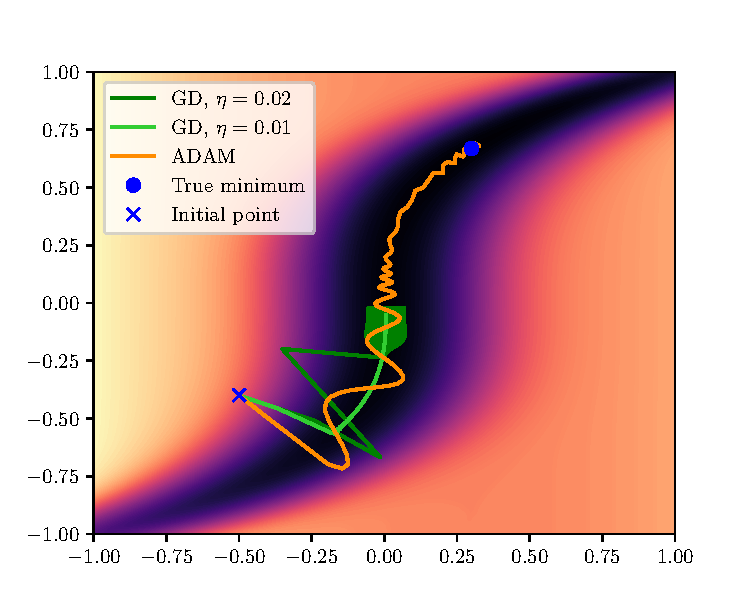
\includegraphics{chapters/theory/adam_vs_gd_plot.pdf}
	\caption{
		A comparison between \gls{adam} and \gls{gd} in an optimization
		landscape with a narrow canyon. The two different \gls{gd} algorithms
		are shown with 1000 steps, while 200 steps with the \gls{adam} algorithm
		are shown.
	}
	\label{fig:adam_vs_gd}
\end{figure}

\todowrt{Pseudocode for the algorithm}
\tododec{Somewhere I should write about epsilon, and alpha and how I set them,
but that probably needs to come later, in the method}
